\section{Road-Quality Vision Model: Fine-Tuning and Evaluation} \label{sec:appx_finetune}

In this section, we document our pipeline to classify road-surface quality from satellite imagery into three classes: poor (0), medium (1), and high (2). We begin from an ImageNet-pretrained vision model called \emph{ConvNeXt V2}, available on \href{https://huggingface.co/docs/transformers/en/model_doc/convnextv2}{Hugging Face} and supported by Meta AI \citep{woo2023convnext}. We use the ConvNeXt V2 backbone and fine-tune the base version of the model on labeled road imagery from \cite{brewer2021}. The resulting model produces categorical ratings which can be converted into a continuous Road Quality Score (RQS), used in Section~\ref{sec:road_quality_decline}.

\paragraph{Fine-tuning Workflow.} Figure~\ref{fig:rq_finetune_flow} summarizes the end-to-end workflow. We begin with a corpus of 53,677 satellite tiles (224x224 pixels) labeled for road quality from \cite{brewer2021}. We feed these images into a ConvNeXt V2 model, replacing the original classification head with a 3-way softmax layer. We then fine-tune the entire model end-to-end using cross-entropy loss and the AdamW optimizer. The training process is monitored via a validation set, and we select the best-performing checkpoint based on minimum validation loss. Finally, we evaluate the fine-tuned model on a held-out test set to report accuracy, F1, and class-wise precision and recall.

\begin{figure}[htbp]
    \centering
    % Replace the file below with your actual flow-chart graphic
    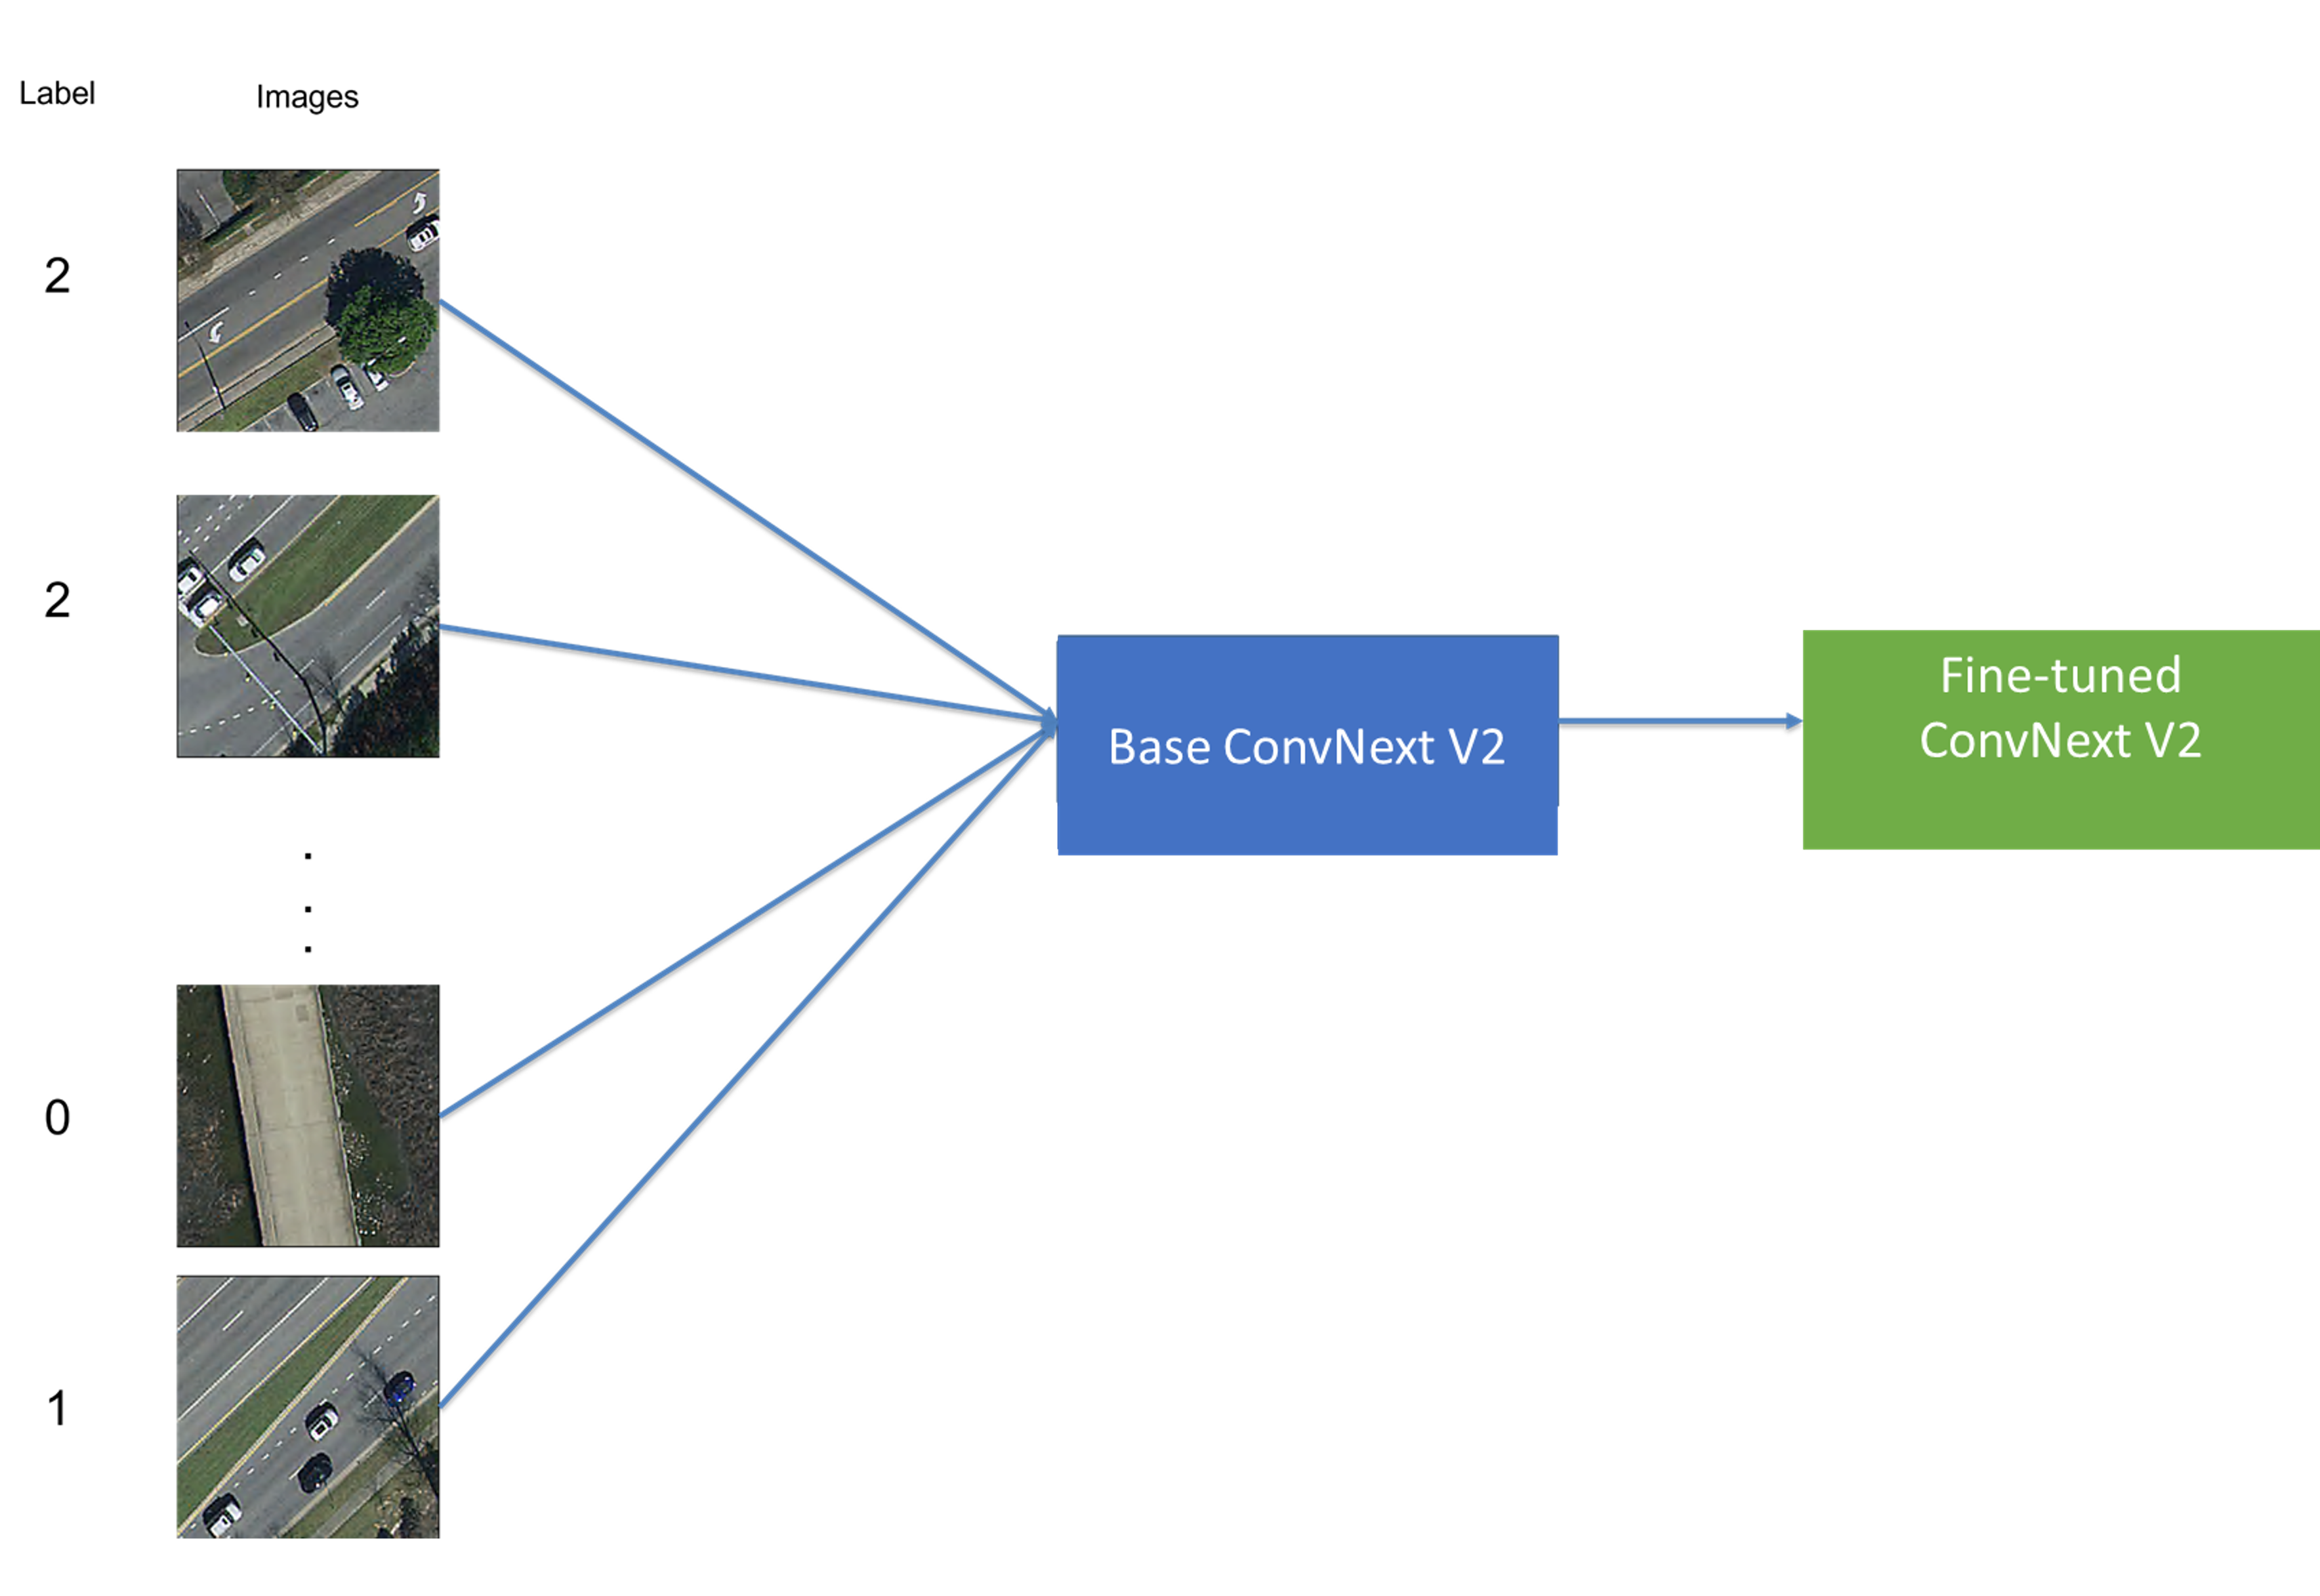
\includegraphics[width=0.92\textwidth,keepaspectratio]{images/fine_tuning_workflow_convnextv2.png}
    \caption{Fine-tuning workflow for road-quality classification}
    \label{fig:rq_finetune_flow}
\end{figure}

% \paragraph{Data and Splits.} We combine labelled satellite tiles from \cite{brewer2021} with Ohio road imagery curated via Google Earth Pro (see Section~\ref{sec:road_quality}). Each image is assigned one of three labels: 0 (poor), 1 (medium), 2 (high). We standardize resolution and apply consistent pre-processing (center-crop, resize, per-channel normalization) to align across sources. We then partition at the jurisdiction (city/township) level to avoid leakage: 70\% train, 15\% validation, 15\% test. The validation set guides hyperparameter selection and early stopping; the held-out test set is reported once at the end.

% \begin{table}[htbp]
%     \centering
%     \caption{Dataset composition and splits}
%     \label{tab:rq_splits}
%     \begin{threeparttable}
%     \begin{tabular}{lrrrr}
%         \toprule
%         & Train & Validation & Test & Total \\
%         \midrule
%         Images & 37{,}574 & 8{,}056 & 8{,}047 & 53{,}677 \\
%         Jurisdictions & 430 & 94 & 93 & 617 \\
%         Class balance (0/1/2) & ~33\%/~34\%/~33\% & ~33\%/~34\%/~33\% & ~33\%/~34\%/~33\% & -- \\
%         \bottomrule
%     \end{tabular}
%     \begin{tablenotes}[flushleft]
%         \footnotesize
%         \item Notes: Example counts illustrate the target 70/15/15 split using the 53{,}677-image corpus from \cite{brewer2021} augmented with Ohio tiles. Jurisdictions are mutually exclusive across splits.
%     \end{tablenotes}
%     \end{threeparttable}
% \end{table}

\paragraph{Data and Training.} We fine-tune ConvNeXt V2 trained on ImageNet-1k dataset. The classification head is replaced by a 3-way softmax. We fine-tune the model for 3 epochs and use cross-entropy loss, AdamW optimizer with learning rate of $5\times10^{-5}$ and weight decay of 0.01, and a batch size of 16 for training and 32 for evaluation. Inputs use the model’s ImageNet normalization; no explicit augmentation. We use a weighted, stratified 70/15/15 split and select the checkpoint with the lowest validation loss.

\begin{table}[h!]
\centering
\small
\begin{tabular}{lccc p{6.8cm}}
\toprule
\textbf{Split} & \textbf{Share} & \textbf{Stratified} & \textbf{Weights} & \textbf{Rationale} \\
\midrule
Train       & 70\% & By label & 3/2/1 & Mitigates class imbalance by allocating more minority-class samples to training, improving gradient signal and stability. \\
Validation  & 15\% & By label & 3/2/1 & Class-aware monitoring consistent with train; used for model selection (min.\ val.\ loss). \\
Test        & 15\% & By label & 3/2/1 & Hold-out evaluation with comparable class mix for fair assessment across splits. \\
\bottomrule
\end{tabular}
\caption{Split design and class-aware allocation. Weights are used only to allocate per-class counts into splits, \emph{not} as loss weights.}
\label{tab:splits}
\end{table}


\paragraph{Model Evaluation Metrics.} We report accuracy, macro F1, and class-wise precision/recall to account for any residual imbalance. We also provide a confusion matrix to diagnose systematic confusions between adjacent quality classes.

\begin{table}[h!]
    \centering
    % \scriptsize
    \caption{Overall accuracy by split (fine-tuned ConvNeXt V2).}
    \begin{tabular}{l c}
        \hline
        Split & Overall Accuracy \\
        \hline
        Train & 0.9115 \\
        Validation & 0.8525 \\
        Test & 0.8337 \\
        \hline
    \end{tabular}
    \label{tab:overall_acc_tiny}
\end{table}

\begin{table}[h!]
  \centering
  \caption{Confusion matrix on the held-out Test set (N=1{,}539). Low/Medium/High correspond to classes 0/1/2.}
  \small
  \begin{tabular}{llccc}
    \toprule
    & & \multicolumn{3}{c}{Predicted} \\
    \cmidrule(lr){3-5}
    & & Low & Medium & High \\
    \midrule
    \multirow{3}{*}{Actual} & Low    & 33 & 11 &  9 \\
                          & Medium & 12 & 78 & 181 \\
                          & High   &  2 & 41 & 1172 \\
    \bottomrule
  \end{tabular}
  \label{tab:rq_confmat_test}
\end{table}


\begin{table}[h!]
    \centering
    \small
    \caption{Classification metrics on the Test set derived from Table~\ref{tab:rq_confmat_test}.}
    \begin{tabular}{lccccr}
        \toprule
        Class & Precision & Recall & F1 & Support \\
        \midrule
        0 & 0.702 & 0.623 & 0.660 & 53 \\
        1 & 0.600 & 0.288 & 0.389 & 271 \\
        2 & 0.861 & 0.965 & 0.910 & 1{,}215 \\
        \midrule
        Macro avg   & 0.721 & 0.625 & 0.653 & 1{,}539 \\
        Weighted avg& 0.810 & 0.834 & 0.810 & 1{,}539 \\
        \midrule
        Accuracy    & \multicolumn{3}{c}{0.8337} & 1{,}539 \\
        \bottomrule
    \end{tabular}
    \label{tab:rq_cls_report_test}
\end{table}

% \paragraph{Split design (Table~\ref{tab:splits}).} The dataset is partitioned 70/15/15 with stratification by label to preserve class proportions. Class-aware allocation weights (3/2/1 for classes 0/1/2) prioritize minority classes during split assignment—especially in training—without altering the loss, yielding balanced monitoring and a fair hold-out test.

Table~\ref{tab:overall_acc_tiny} presents model accuracy results on training, validation and test datasets. Accuracy is 0.9115 on train, 0.8525 on validation, and 0.8337 on test, indicating a good fit without overfitting on training data. As expected, accuracy declines slightly from train to validation to test. However, the gap between validation and test is less than 10 percentage points, suggesting good generalization across unseen data. 

Table~\ref{tab:rq_confmat_test} shows the confusion matrix on the held-out test set and is useful to understand the types of errors the model makes when classifying road quality. As presented in the table, most errors are between adjacent classes: medium (1) is often predicted as high (2), and poor (0) occasionally as medium (1). Confusions between poor (0) and high (2) are rare, while high (2) is predominantly classified correctly.

Table~\ref{tab:rq_cls_report_test} presents per-class metrics. Class 2 attains high precision and recall, driving weighted averages near overall accuracy, which suggests the model is very reliable at identifying high-quality roads. Class 1 shows low recall, lowering macro F1 and reflecting difficulty on borderline surfaces. This means the model often misses medium-quality roads, misclassifying them as high quality. Class 0 performs moderately, with balanced precision/recall relative to its smaller support, indicating reasonable reliability on poor-quality roads despite fewer examples. Overall, the model excels at identifying high-quality roads but nevertheless struggles more with medium and poor classes, especially in recall for medium quality.

% \begin{figure}[htbp]
%     \centering
%     % Replace with your actual confusion-matrix image
%     \includegraphics[width=0.65\textwidth,keepaspectratio]{images/rq_confusion_matrix.png}
%     \caption{Confusion matrix on the held-out test set. Most errors occur between adjacent categories (1 vs 2; 0 vs 1), consistent with visual continuity of surface wear.}
%     \label{fig:rq_confmat}
% \end{figure}

\paragraph{Base vs. Fine-Tuned ConvNeXt V2.} Table~\ref{tab:rq_perf} summarizes the main gains from end-to-end adaptation. We compare our fine-tuned ConvNeXt V2 against a baseline where the pretrained backbone is frozen and only the classification head is trained. This linear-probe baseline on frozen ImageNet features approach is common in transfer learning.

\begin{table}[h!]
\centering
% \small
\caption{Fine-tuned vs. baseline ConvNeXt V2.}
\label{tab:rq_perf}
\begin{tabular}{lc}
    \toprule
    Model & Overall Accuracy \\
    \midrule
    Fine-tuned ConvNeXt V2 & 0.8337 \\
    Baseline ConvNeXt V2   & 0.2586 \\
    \bottomrule
\end{tabular}
\end{table}

Fine-tuning improves test accuracy by 57.51 (from 0.2586 to 0.8337) percentage points, a more than 220\% relative gain. This indicates that adapting the pretrained backbone to road imagery is crucial for learning task-specific features and achieving reliable generalization, justifying end-to-end fine-tuning over a frozen baseline.

% \paragraph{Implementation Notes.} Images are referenced by path and identifier, with per-sample metadata (jurisdiction, capture year) used to enforce split integrity and to align pre/post referendum windows. To ensure reproducibility, seeds were fixed for data shuffling and weight initialization, and we logged runs (metrics and artifacts) for auditability.
